%!TEX root = ../../main.tex
\section{Extrapolation routine}
\label{sec:Extrapolation routine}

\subsection{Regression extrapolation}
\label{sub:Regression extrapolation}
With both the reflection intensities and the doses extracted, extrapolation can be performed using standard regression techniques.
In particular, parametric regression in which a particular functional form describing the relationship between the two variables was implemented.
The function chosen to describe the relationship between the reflection intensity, $I$, and the dose, $D$, was:
\begin{equation}
    I_{calc}(D) = K_{\bs{h}} \exp \left[- A^2_{\bs{h}}D^2 - B_{\bs{h}}D h^2/2 \right]
    \label{eq:Extrapolation regression function}
\end{equation}
Where $\bs{h}$ represents the miller indices of a reflection, $h = |\bs{h}| = 1/d$, where $d$ is the spacing between adjacent Bragg planes and $K_{\bs{h}}, A_{\bs{h}}, B_{\bs{h}}$ are reflection specific parameters to be determined.
Note that this equation is identical to the Leal \textit{et al.} model (equations \ref{eq:Leal DDM}, \ref{eqscale} and \ref{eqB}) where
\begin{align}
    A^2_{\bs{h}} &= \gamma^2, \\
    B_{\bs{h}} &= \beta, \\
    K_{\bs{h}} &= K\exp \left[ -B_0 h^2/2 \right].
\end{align}
Essentially equation \ref{eq:Extrapolation regression function} is a Gaussian function.
Hence the Leal \textit{et al.} model describes a Gaussian decay of reflection intensity with the dose.
The values of the parameters $K_{\bs{h}}, A_{\bs{h}}$, and $B_{\bs{h}}$ will determine which section of the Gaussian will best describe the change in intensity for a given reflection.

To determine the parameter values (and hence the decay of intensity of a reflection), all observations of equivalent\footnote{Equivalent in this sense means all symmetry equivalents and Friedel pairs} reflections were grouped together to form the set of observed intensities.
The parameter values were then found as the values that minimised the function
\begin{equation}
\sum_{obs} w_{obs}\left(I_{obs}(D_{obs}) - I_{calc}(D_{obs}) \right)^2
\label{eq:Extrapolation objective function}
\end{equation}
Where $w_{obs} = 1/\sigma_{obs}^2$ is the weighting term and $\sigma_{obs}$ is the standard deviation of the observation, $I_{obs}(D_{obs})$ is the observed intensity value at dose $D_{obs}$.
The optimization routine is performed using the MATLAB \verb|fminsearch| routine which uses the simplex search method of Lagarias et al. \cite{lagarias1998convergence}.
This is a direct search method that does not use numerical or analytic gradients.

To ensure that the \verb|fminsearch| routine converges to sensible final parameter values, it needs to be seeded with suitable initial guesses of the values. To create the initial guesses, 3 observations (first, last and an observation from the middle of a dataset - provided they meet the criteria mentioned in the rest of this section) are used to analytically find the parameter values such that the function passes through all three points.

One of the main problems with obtaining accurate data in crystallography is the limited multiplicity of reflection observations.
This can also be problematic for performing accurate regression.
Equation \ref{eq:Extrapolation regression function} requires three parameter values, therefore there should be at least three observations to perform extrapolation.
However with only three observations, the regression is likely to lead to overfitting of the model to the data (Figure~\ref{fig:Data Overfitting to few data points - Extrapolation method}).
To prevent overfitting a minimum of 6 observations was required before extrapolation was performed.
\begin{figure}
  \centering
    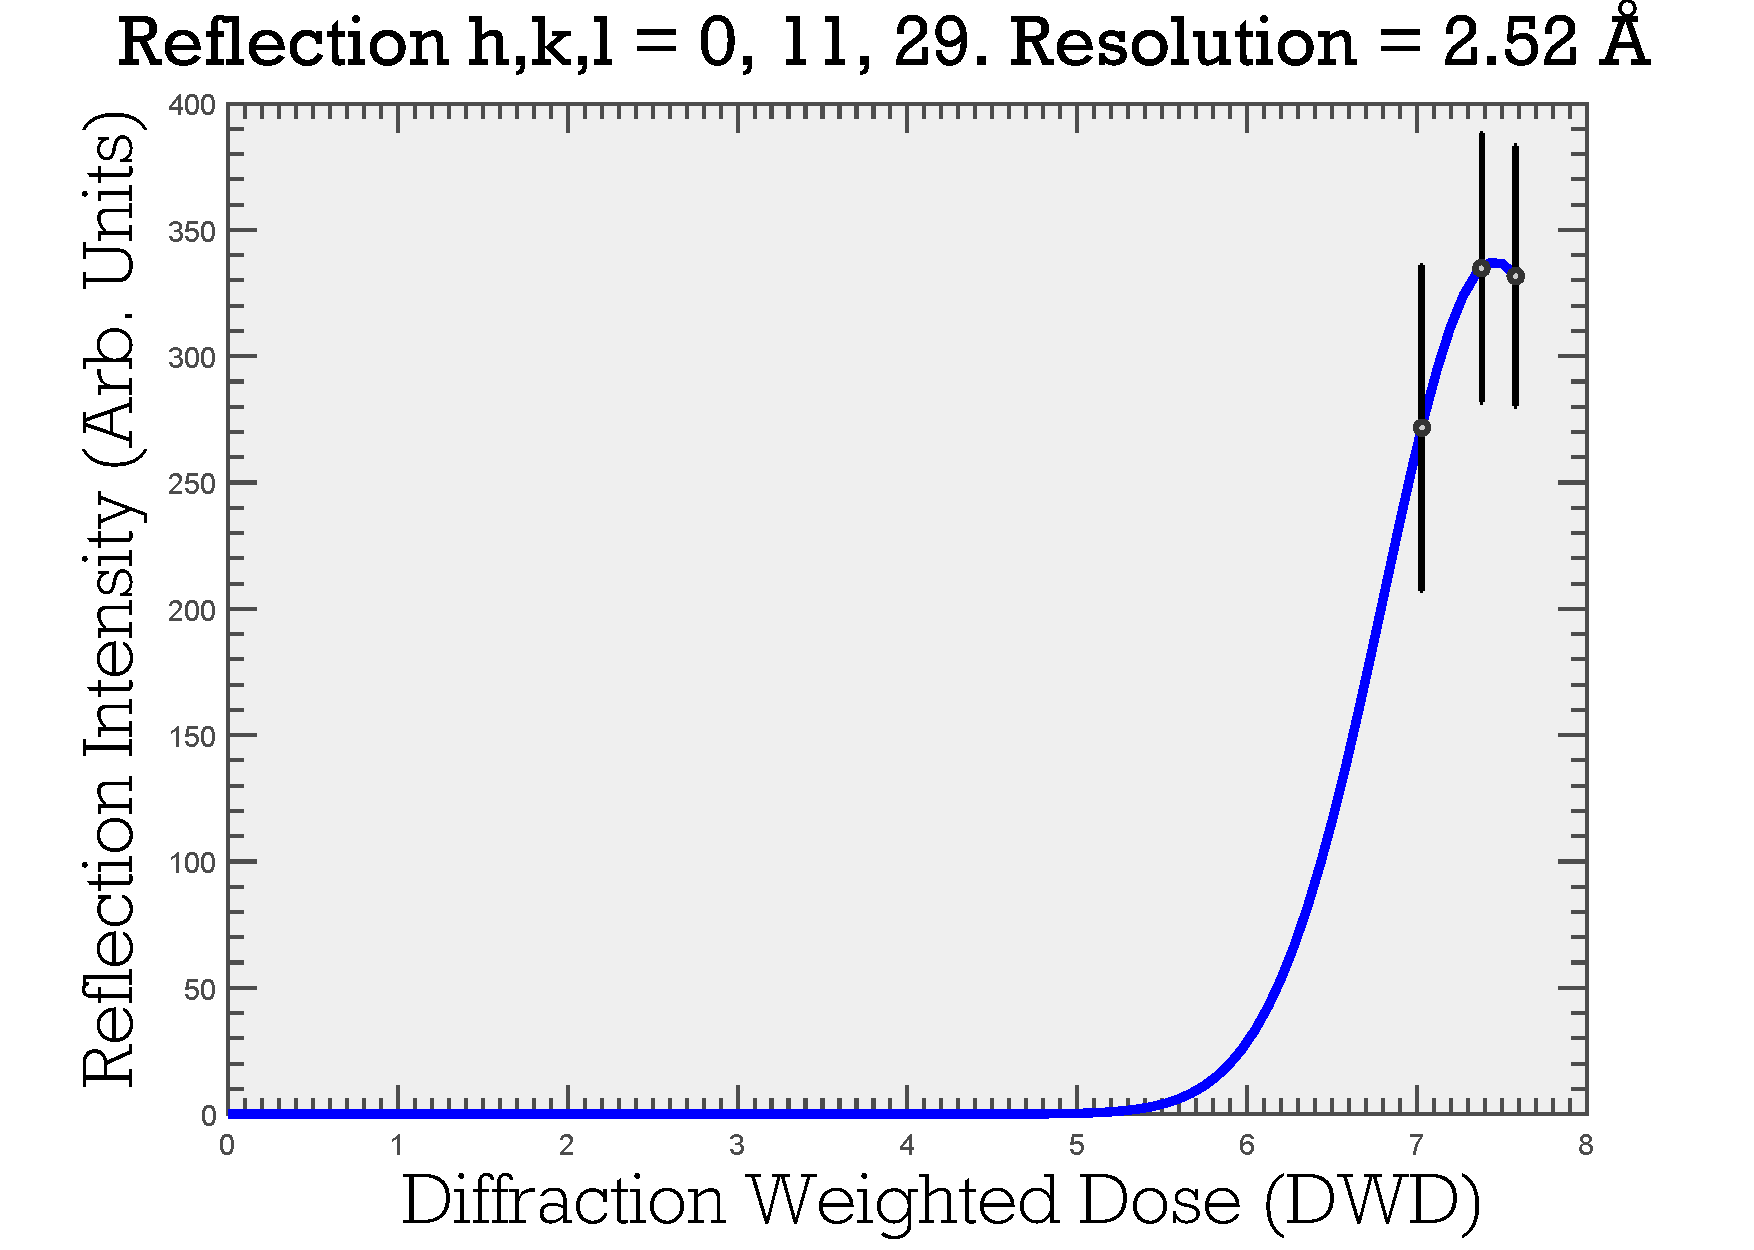
\includegraphics[width=1\textwidth]{figures/zde/ReflectionPlot_h,k,l_0,11,29-3obs.pdf}
    \caption{Regression performed where the model has been overfitted to the data.
    The function passes perfectly through all three data points but predicts a zero-dose intensity of zero.}
    \label{fig:Data Overfitting to few data points - Extrapolation method}
\end{figure}

An additional procedure to prevent overfitted was to ensure that the fit correlated with the data.
Therefore after the regression was performed, a correlation coefficient was calculated between the model fit and the data.
If the resulting correlation was below a specified value (0.5 was chosen acceptable then the extrapolation was not performed.
A bad correlation suggested that there were problems with the fit as in Figure~\ref{fig:Bad correlation bad fit - Extrapolation method} where the correlation coefficient was 0.209.
However a bad correlation value did not always suggest a bad fit as shown in Figure~\ref{fig:Bad correlation good fit - Extrapolation method}, where the correlation was  quite low (0.231) but the fit looks reasonably good when accounting for the noise level.
\begin{figure}
        \centering
        \begin{subfigure}[b]{1\textwidth}
                \centering
                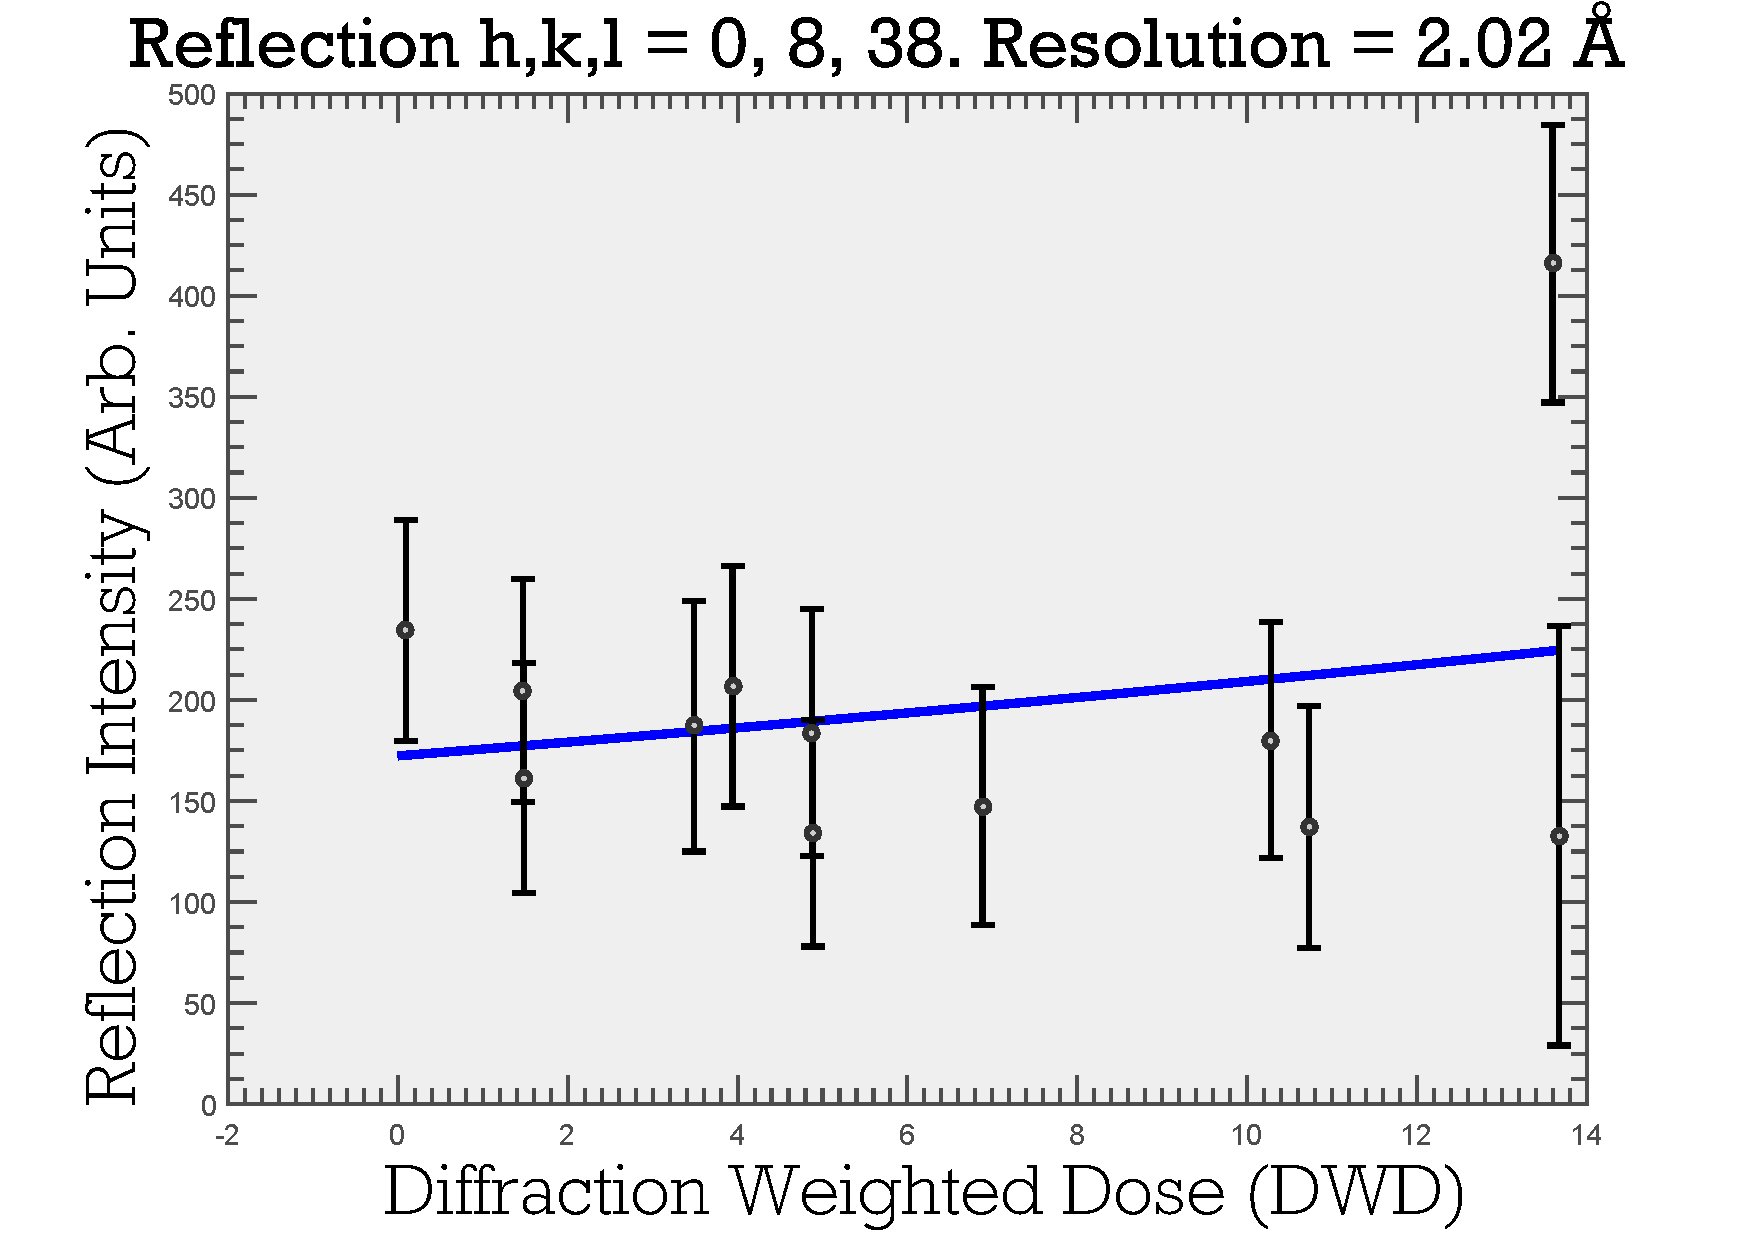
\includegraphics[width=\textwidth]{figures/zde/ReflectionPlot_h,k,l_0,8,38-bad_corr_bad_fit.pdf}
                \caption{}
                \label{fig:Bad correlation bad fit - Extrapolation method}
        \end{subfigure}
				\\
        \begin{subfigure}[b]{1\textwidth}
                \centering
                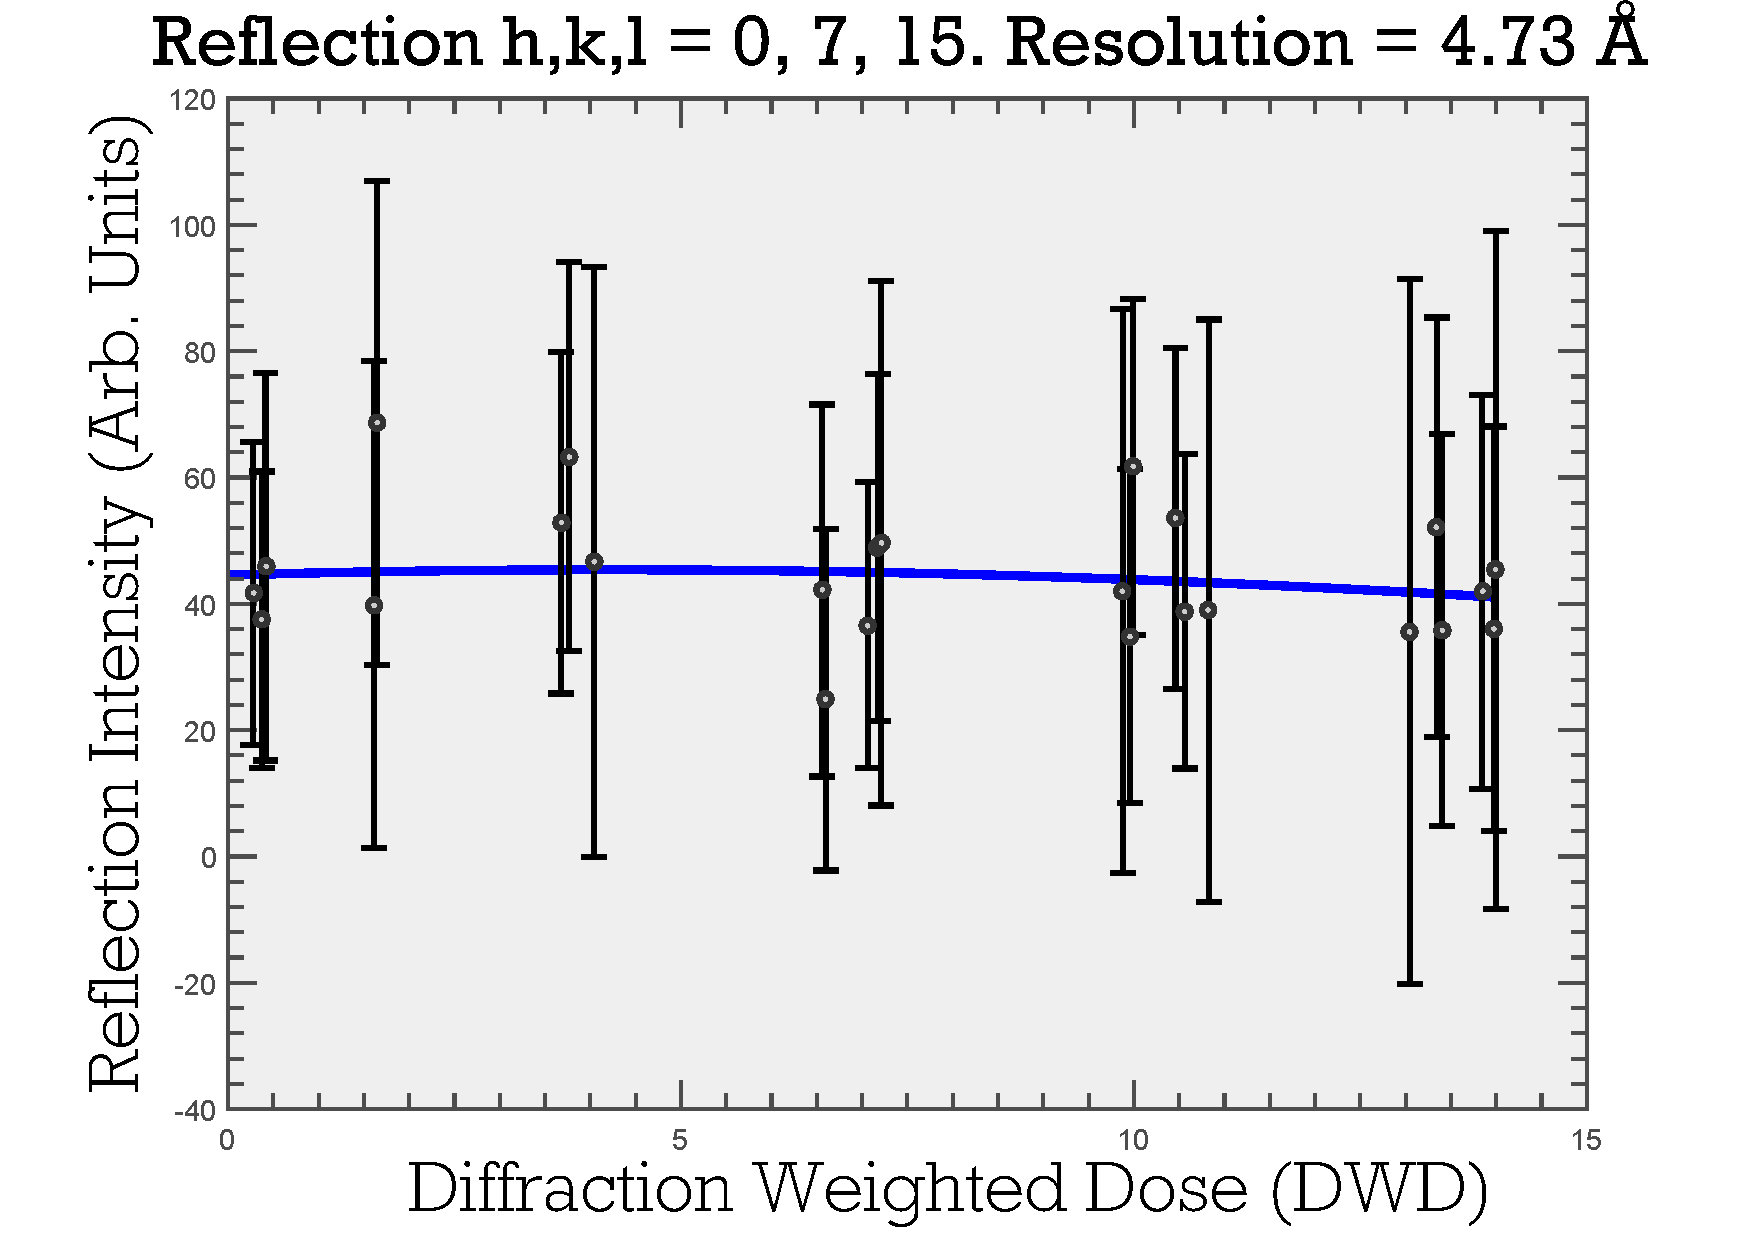
\includegraphics[width=\textwidth]{figures/zde/ReflectionPlot_h,k,l_0,7,15-bad_corr_good_fit.pdf}
                \caption{}
                \label{fig:Bad correlation good fit - Extrapolation method}
        \end{subfigure}
        \caption{(a) Regression performed for a reflection where the correlation coefficient was determined to be 0.209.
        The bad correlation coefficient is consistent with the bad fit of the model to the data.
        (b) Regression performed for a reflection where the correlation coefficient was determined to be 0.231.
        The bad correlation coefficient in this case is clearly due to the noisy measurements but the fit looks to give sensible intensity predictions that are consistently within the standard deviation of every observation.}
        \label{fig:Bad correlation plots - Extrapolation method}
\end{figure}

Other checks were also performed to make sure that the resulting fits and zero-dose extrapolated intensities were reasonable:
\begin{enumerate}
    \item check that the first $M$ observations are significantly above zero, where $M$ is a user defined value which was set to 6.
    The exact procedure was to check that for the first $M$ observations $I_{obs}(D_{obs}) - n_0\sigma_{obs} > 0$, where $n_0 = 0.5$.
    This was done to prevent overfitting that could result from trying to fit to very small or negative values as exemplified in Figure~\ref{fig:Data overfitting to small values - Extrapolation method}.
    The reason that the fit is bad is because the Leal \textit{et al.} model is always positive for any positive real-valued dose.
    Hence fitting the function to small or negative values is likely to result in an untrustworthy fit.
    \item the calculated zero-dose intensity using the fitted parameter values gives a finite value and it is not significantly larger than the intensity values from the rest of the dataset.
    This is to prevent unreasonable fits as shown in Figure~\ref{fig:Unphysically high zero-dose intensity - Extrapolation method}.
\end{enumerate}

\begin{figure}
        \centering
        \begin{subfigure}[b]{1\textwidth}
                \centering
                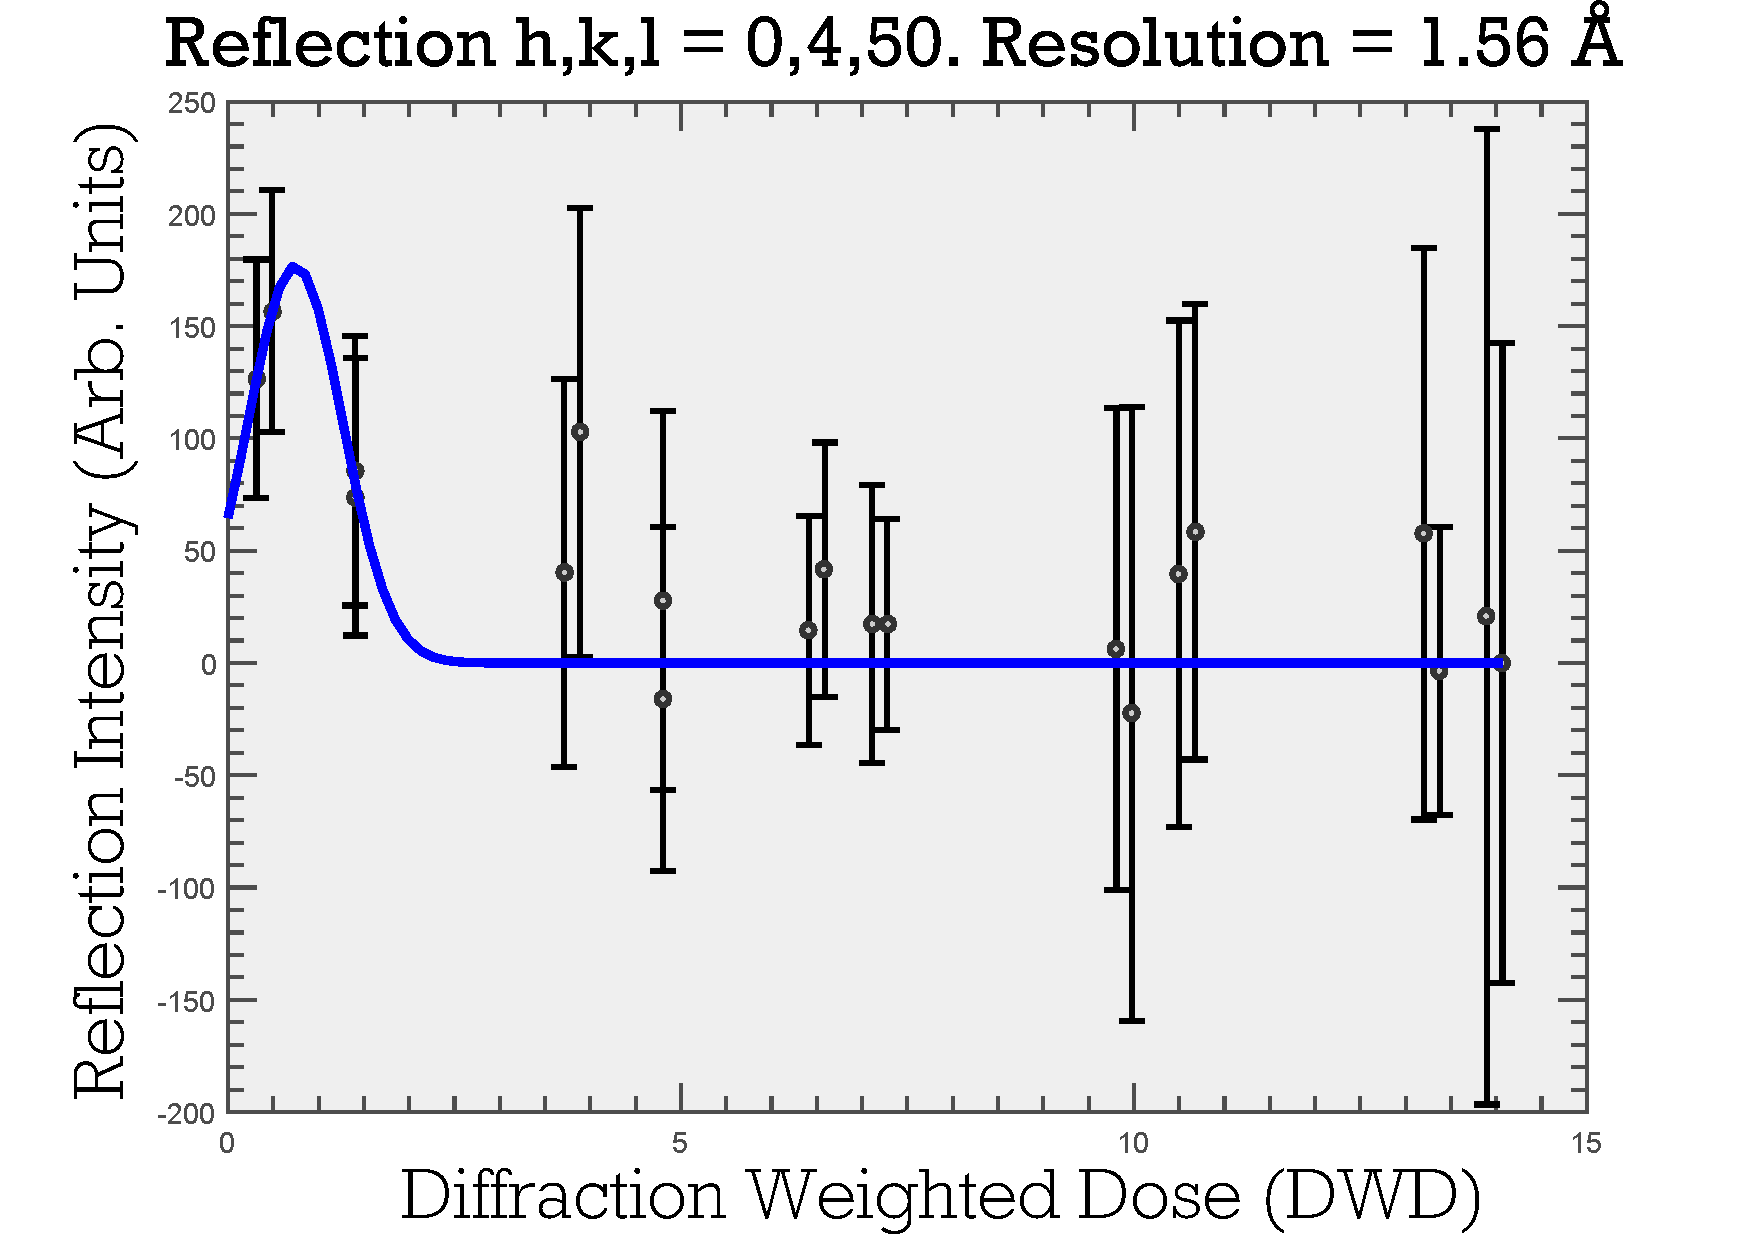
\includegraphics[width=\textwidth]{figures/zde/ReflectionPlot_h,k,l_0,4,50_fit_to_small_values.pdf}
                \caption{}
                \label{fig:Data overfitting to small values - Extrapolation method}
        \end{subfigure}
				\\
        \begin{subfigure}[b]{1\textwidth}
                \centering
                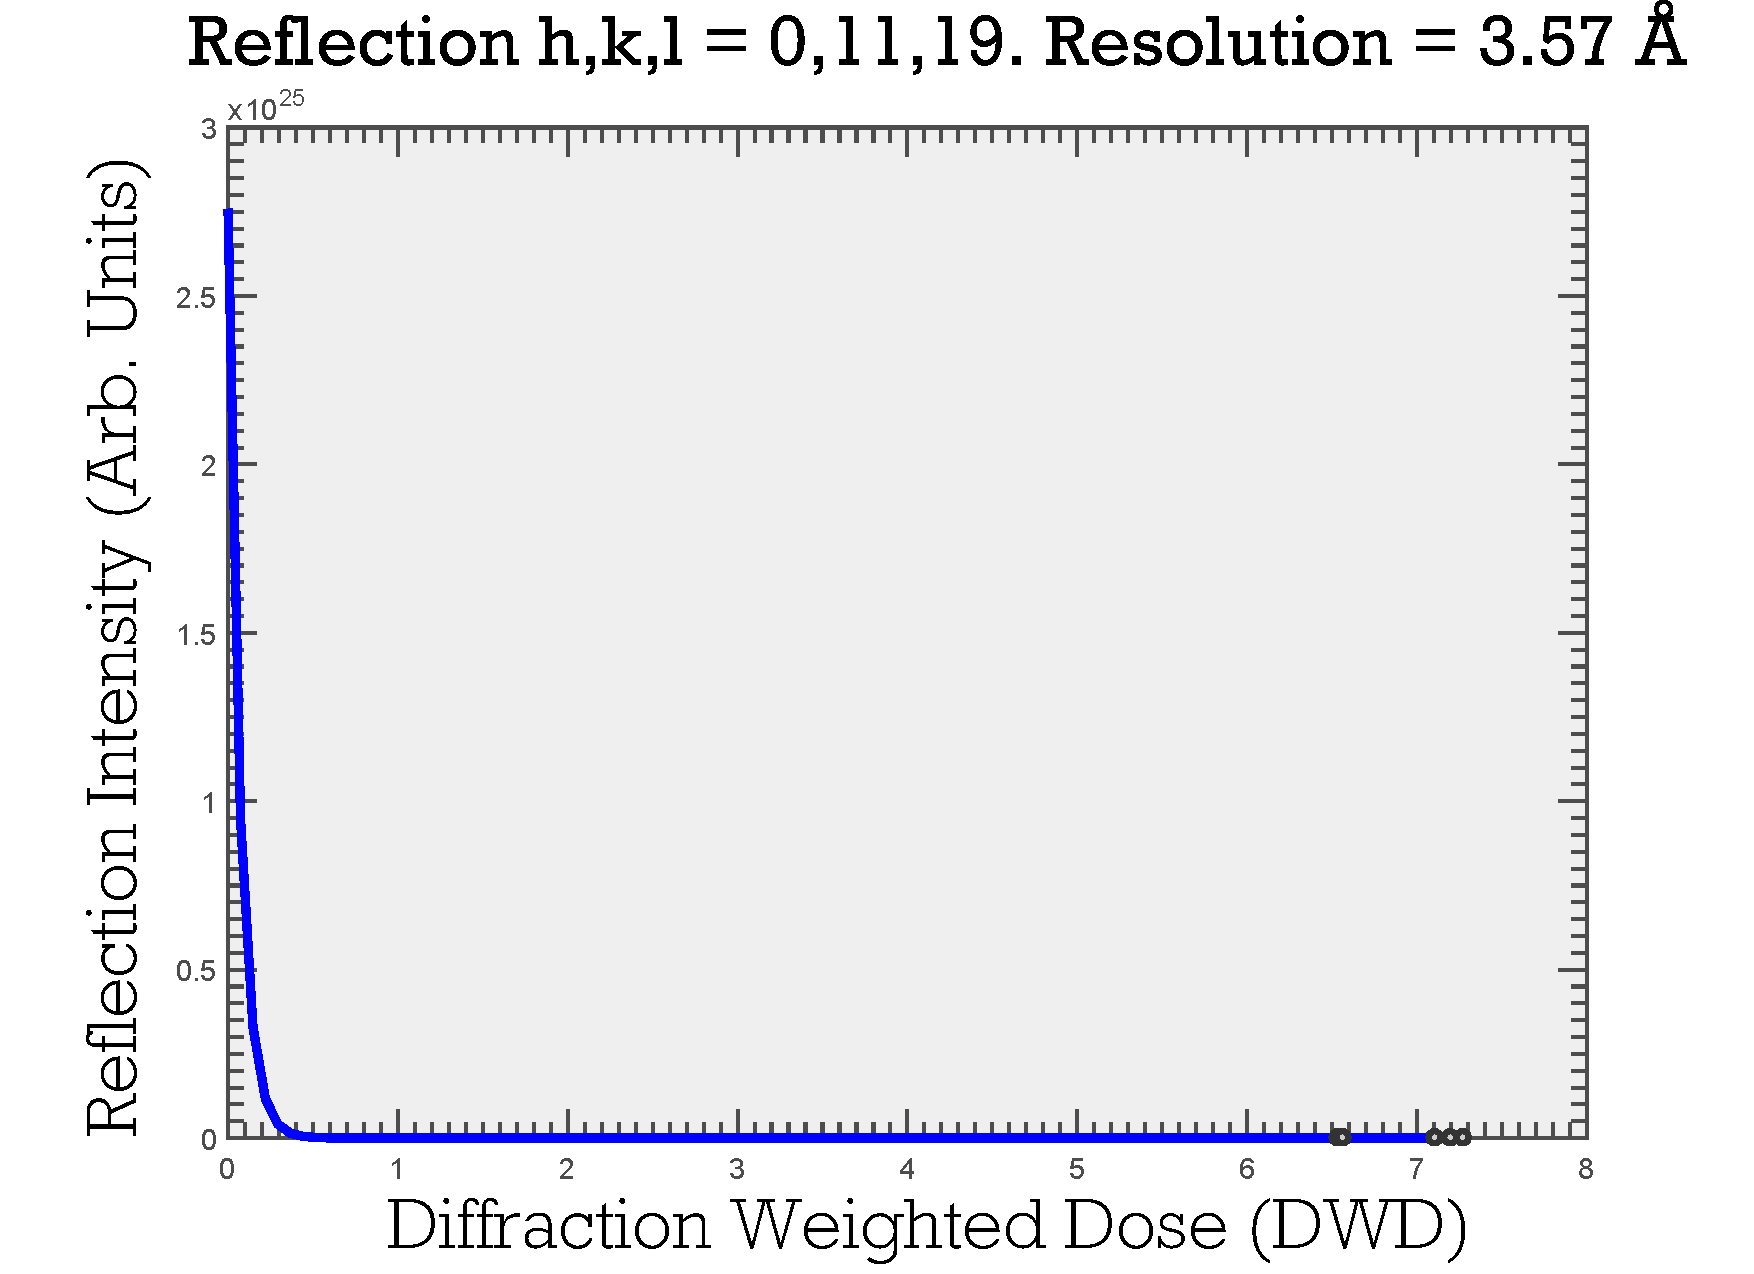
\includegraphics[width=\textwidth]{figures/zde/ReflectionPlot_h,k,l_0,11,19_zero_dose_too_high.pdf}
                \caption{}
                \label{fig:Unphysically high zero-dose intensity - Extrapolation method}
        \end{subfigure}
        \caption{(a) Overfitting as a result of fitting equation \ref{eq:Extrapolation regression function} to data where the values are too small or negative.
        Equation \ref{eq:Extrapolation regression function} is always positive for all positive real-valued dose values so the fit is very bad when observations are too small.
        (b) A zero-dose estimate that is unphysically high despite a good fit to 5 data points.
        This often happens when the only observations of a reflection occur relatively close to each other but far away from the zero-dose state.}
        \label{fig:Bad Extrapolations, violated checks - Extrapolation method}
\end{figure}

All of the above checks are made to ensure that the model fit is representative of the data.
However the zero-dose values are not obtained from these fits (i.e. the zero dose value of the blue line in Figures~\ref{fig:Data Overfitting to few data points - Extrapolation method}, \ref{fig:Bad correlation plots - Extrapolation method} and \ref{fig:Bad Extrapolations, violated checks - Extrapolation method}).
Instead the zero dose value is obtained separately for each reflection to preserve the spread of the data for rescaling.
This is exactly the same method used by Diederichs \textit{et al.} \cite{diederichs2003}.
To obtain the zero-dose estimate for each observation, $K_{\bs{h}}$, equation \ref{eq:Extrapolation regression function} is rearranged to get
\begin{equation}
    K_{\bs{h}} = \exp\left[\log(I_{obs}(D_{obs})) + A^2_{\bs{h}}D^2_{obs} + B_{\bs{h}} D_{obs} h/2\right].
    \label{eq:Zero-dose extrapolated intensity for each reflection observation}
\end{equation}

Although the zero-dose observations are estimated using regression analysis, the standard deviations are not dealt with by this method.
The standard deviation is computed as
\begin{equation}
    \sigma^{corr}_{\bs{h}} = \sqrt{\sigma^2_{obs}(1 + D^2_{min})}
    \label{eq:Corrected sigma value - Extrapolation method}
\end{equation}
where $\sigma_{corr}$ is the corrected $\sigma$ value, $\sigma_{obs}$ is the observed $\sigma$ value and $D_{min}$ is the dose value of the first observation.
Equation \ref{eq:Corrected sigma value - Extrapolation method} takes the same form as the corrected standard deviation in \cite{diederichs2003}, with a couple of differences:
\begin{enumerate}
    \item the standard deviation is inflated by the addition of a term which involves the standard deviation a decay factor which is assumed common to all observations in a dataset.
    Because a different decay formed is used for the extrapolation in the current work there is no single term which is directly analogous to the decay factor.
    \item $D_{min}$ is used instead of the actual dose of the crystal during the observation because I believe a big factor in the reliability of the extrapolation is how early the initial measurement was made.
    A thought experiment to see this is to suppose a reflection is observed on every frame in a MX experiment where the dose range is 1-10 MGy, and another reflection is observed on every frame from a dose of 5.5 MGy onwards.
    Assume that observations of these reflections on the same image have the same sigma values.
    It is also assumed that the regression fits are theoretically perfect for both reflections.
    In the case where the dose value at which the observation was made is used to inflate the standard deviations, the inflated values for the extrapolation of the observations will have the same value.
    This is despite the fact that one of the reflections was only initially observed half way through the experiment.
    In the case where the reflection was only observed half way through the experiment, I believe that the zero-dose value should have a higher uncertainty than the zero-dose value for the reflection that was observed from the first frame regardless of the dose at which an observation is made.
\end{enumerate}

\subsection{Probabilistic extrapolation}
\label{sub:Probabilistic extrapolation}
The regression analysis performed as described above requires several checks to be made to ensure that the model fit to the data is reasonable.
This essentially filters out reflections that do not behave according to the relationship expected by equation \ref{eq:Extrapolation regression function}, so some reflections are not extrapolated.
Therefore Bayesian inference is used to extrapolate these remaining reflections.
Bayes theorem in model form states
\begin{equation}
P(model|data) \propto P(data | model) \times P(model),
\label{eq:Bayesian Theorem in model form}
\end{equation}
where $P(model|data)$ is the posterior distribution, the updated probability of the model given the observed data, $P(data|model)$ is the likelihood function, the probability of observing the data given the current model, and $P(model)$ is the prior distribution, which represents the probability of the model in the absence of any data.
In this case, the $model \equiv J$, where $J$ is the expected intensity, and $data \equiv I, D$ where $I$ represent the observed intensity and $D$ the observed dose.

$P(J|I,D)$ is the distribution of interest because this will give the probability of an observation having a particular intensity value, $J$, given the intensity observed, $I$, at a particular dose, $D$.
The expected value of this distribution will be the extrapolated intensity value.
The expected value is given by
\begin{equation}
    E(J|I, D) = \int_0^{\infty} J \times P(J|I,D)\, \mathrm{d}J.
    \label{eq:Expected intensity value - Extrapolation method}
\end{equation}
Furthermore the variance if the observation can be obtained from the posterior distribution as
\begin{equation}
    var(J|I, D) = \int_0^{\infty}  \left( J - E(J|I, D) \right)^2 \times P(J|I,D)\, \mathrm{d}J
    \label{eq:Variance of intensity value - Extrapolation method}
\end{equation}
Therefore the likelihood $\equiv P(I | J, D)$ and prior $\equiv P(J)$ distributions are thus required to calculate the posterior distribution.

The prior, $P(J)$, is given by the Wilson distribution for intensities \cite{wilson1949probability}.
For acentric reflections the Wilson distribution is
\begin{equation}
    f(n) =
    \begin{cases}
        (\varepsilon_{\bs{h}}\Sigma)^{-1} \exp(-J/\varepsilon_{\bs{h}}\Sigma) & \mbox{if } J \ge 0, \\
        0                           & \mbox{if } J < 0,
    \end{cases}
    \label{eq:Wilson Distribution for acentric reflections - Intensities}
\end{equation}
whereas for centric reflections it is
\begin{equation}
    f(n) =
    \begin{cases}
        (2\pi\varepsilon_{\bs{h}}\Sigma J)^{-1/2} \exp(-J/2\varepsilon_{\bs{h}}\Sigma) & \mbox{if } J \ge 0, \\
        0                                      & \mbox{if } J < 0,
    \end{cases}
    \label{eq:Wilson Distribution for centric reflections - Intensities}
\end{equation}
where $\Sigma$ is the distribution parameter, which here represents the mean intensity in the corresponding resolution shell of reciprocal space and $\varepsilon_{\bs{h}}$ is the multiplicity of the reflection with reciprocal lattice vector $\bs{h}$. $\varepsilon_{\bs{h}}$ is an integer value and the multiplication with $\Sigma$ is to account for the increase in the expected intensity due to the space group symmetry \cite{blessing1998intensity}. A rule for calculating $\varepsilon$ is proposed by Stewart and Karle (1976) \cite{stewart1976}: ``$\varepsilon$ is the number of times the transformed vector, $\bs{h}_t = (h,k,l)_t$, is identical to a given reflection, $\bs{h} = (h,k,l)$, under all distinct pure rotational symmetry operations $\bs{R}$ of the space group; $\bs{h}_t = \bs{h}\bs{R}_t$.''
The mean intensity of a resolution bin, $\Sigma$ must be corrected for $\varepsilon$.
Therefore, the mean intensity of a resolution bin is given by
\begin{equation}
    \Sigma = <I/\varepsilon> = \f{\sum^{n_{bin}}_i I^i_{\bs{h},obs}/\varepsilon_{\bs{h}}}{n_{bin}},
    \label{eq:Mean intensity of resolution bin}
\end{equation}
where $n_{bin}$ is the number of reflection observations in a resolution shell and $I^i_{\bs{h},obs}$ is the intensity if the $i^{\text{th}}$ reflection observation with reciprocal lattice vector $\bs{h}$.

It should be noted here that since the aim is to extract the zero dose intensity of observations, the mean intensity value in the resolution bins, $\Sigma$, are not calculated from the intensity measurements of the data.
Instead they are calculated from the zero dose values that were calculated from the regression analysis.

Now that the prior distribution has been specified, it is left to specify the likelihood distribution, $P(I | J, D)$.
In exactly the same approach used in the French and Wilson truncation algorithm, the likelihood is assumed to be a normal distribution.
The main difference is that the intensity data is assumed to have been changed by a scale factor, $s$, which is a function of the dose, $D$.
Therefore the intensity of an observation is normally distributed:
\begin{equation}
    I_{obs} \quad \text{\textasciitilde} \quad N(Js(D_{obs}),\sigma_{obs}^2).
    \label{eq:Normally distributed intensity - Extrapolation method}
\end{equation}
Or more explicitly
\begin{equation}
    P(I_{obs} | J, D_{obs}) = \f{1}{\sigma_{obs} \sqrt{2\pi}} \exp \left[-\f{(I_{obs} - J s(D_{obs}))^2}{2 \sigma^2_{obs}} \right].
    \label{eq:Normally distributed intensity full equation - Extrapolation method}
\end{equation}

So all that remains is to find $s(D)$.
